\documentclass{beamer}
\usepackage[T2A]{fontenc}
\usepackage[utf8]{inputenc}
\usepackage[english,russian]{babel}
\usepackage{graphicx}

\usepackage{beamerthemesplit} % new
\usetheme{Goettingen}
\usecolortheme{seahorse}
% \usefonttheme{structureitalicserif}
\hypersetup{unicode=true}

% \usepackage[unicode]{hyperref}

\begin{document}
\title{Разработка алгоритма для выделения частовстречающихся шаблонов
      ошибок из файлов журналов приложений}
\author{Андрей Тропин}

\institute{
  К06-682 \\
  НИЯУ МИФИ \\
  Москва \\
  \texttt{andrewtropin@gmail.com}
}

\date{\today}

\frame{\titlepage}

% \frame{\frametitle{Содержание}\tableofcontents}


\section{Постановка задачи}
\subsection{Цель работы}

\frame{
  \frametitle{Цель работы}
  \begin{block}{}
Цель работы --- разработка алгоритма для выделения частовстречающихся шаблонов
ошибок из файлов журналов приложений для повышения скорости реакции
на непредвиденные ситуации и повышения стабильности работы распределённой
системы.
  \end{block}
}

\subsection{Задачи}
\frame{
  \frametitle{Задачи}
  Реализовать следующие возможности:
  \begin{itemize}
    \item Хранение и версионирование шаблонов
    \item Получение контекста для шаблона
    \item Подсчёт статистики совпадений
    \item Выделение ``неизвестных`` ранее ошибок
    \item Добавление нового шаблона к существующим
    \item Автоматическое выделение нового шаблона
  \end{itemize}
}
\section{Реализация}
\subsection{Алгоритм}
\frame{
  \frametitle{Краткое описание алгоритма}
    \begin{column}{.94\textwidth}
      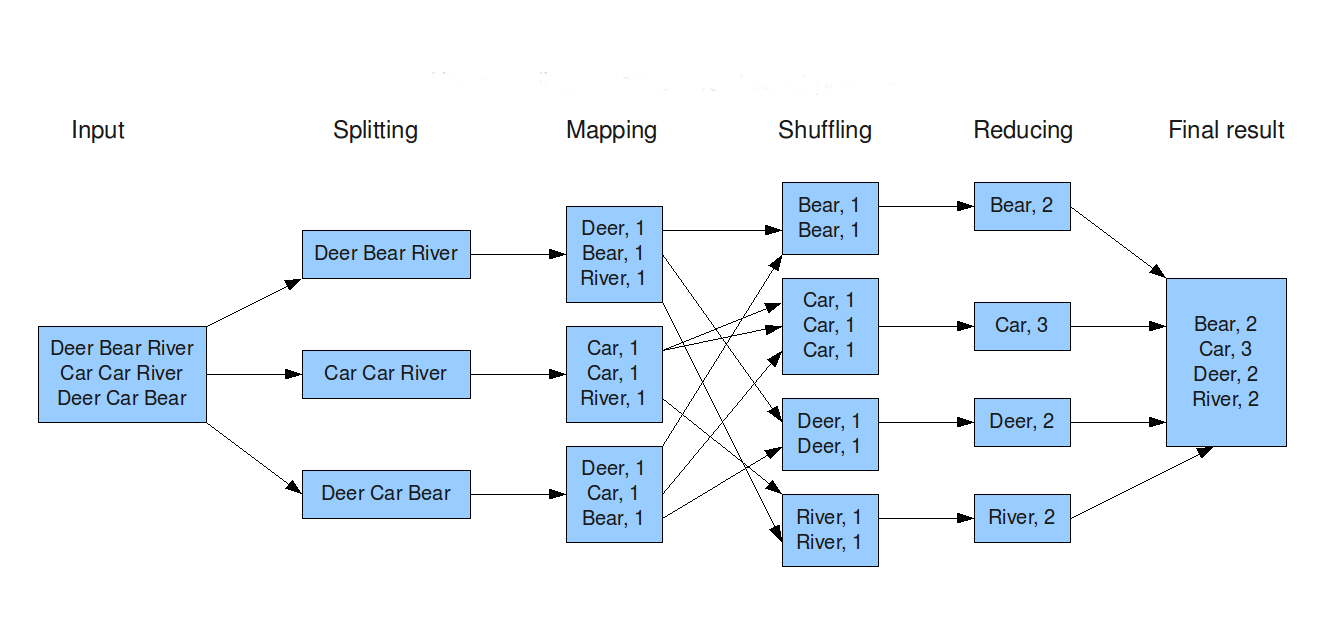
\includegraphics[width=\textwidth]{../report/pics/mapreduce.png}
    \end{column}
}

\subsection{Пример использования}
\frame{
  \frametitle{Пример использования}
    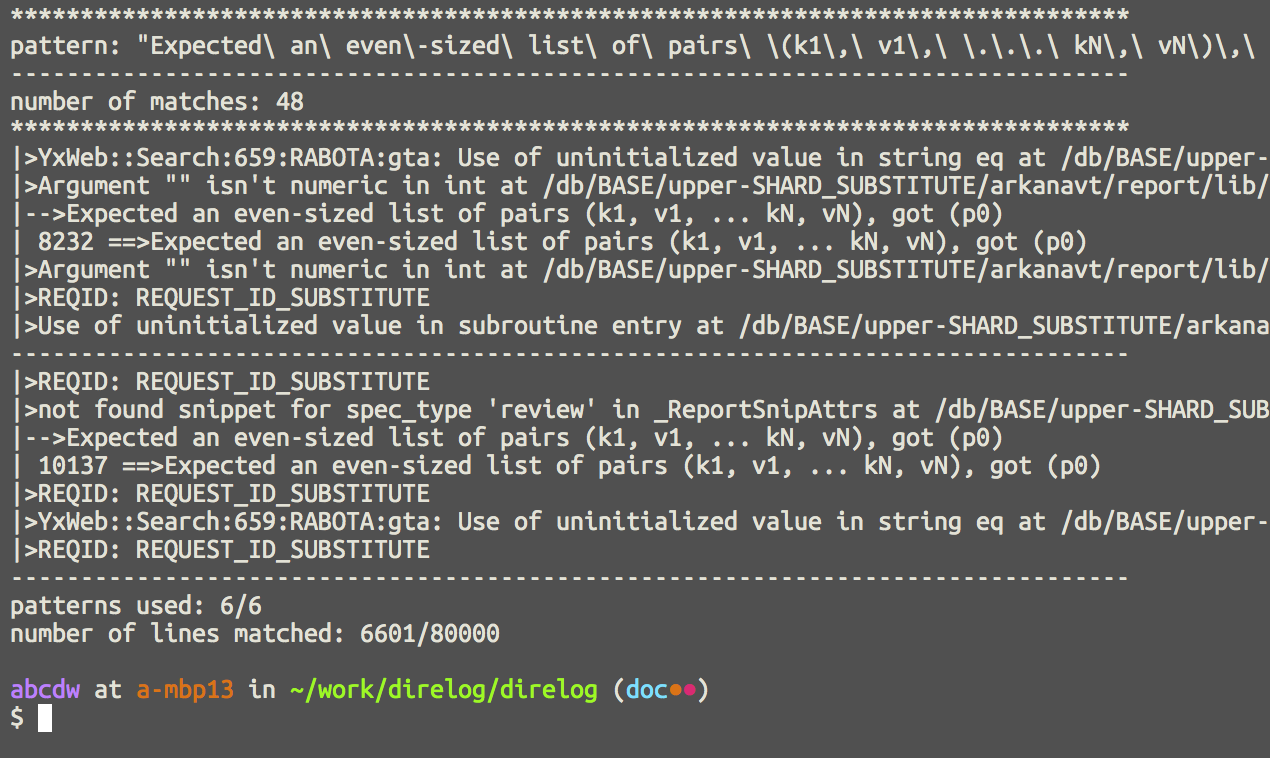
\includegraphics[width=\textwidth]{./direlog.png}
  % \begin{itemize}
    % \item
  % \end{itemize}
}

\section{Результаты}
\subsection{Итог работы}
\frame{
  \frametitle{Итог работы}
  \begin{itemize}
    \item Разработано алгоритм и реализован на языке python
    \item Приложение внедрено в поисковой инфраструктуре.
    \item Благодаря наглядной статистике форсирован рефакторинг подсистемы
      отладочного вывода.
    \item Уменьшен объем отладочных данных генерируемых в единицу времени.
    \item Уменьшено время ручного анализа файла журнала инженером.
    \item Не реализовано автоматическое выделение шаблонов.
  \end{itemize}
}

\subsection{Дальнейшие действия}
\frame{
  \frametitle{Дальнейшие действия}
  \begin{itemize}
    \item Применение машинного обучения для реализации автоматического
      выделения шаблонов.
  \end{itemize}
}

\section{Конец}
\frame{
  \frametitle{Конец}
  \begin{center}
    Спасибо за внимание.
  \end{center}
}

\end{document}

